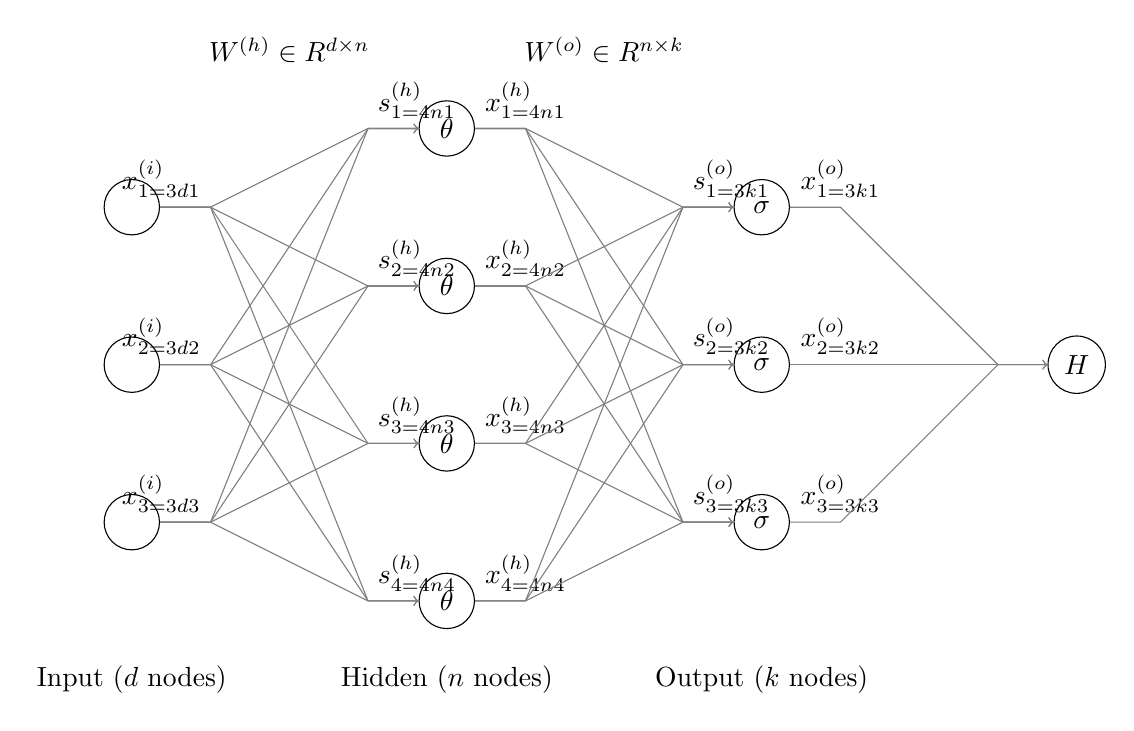
\begin{tikzpicture}[->,draw=black!50]
\tikzstyle{neuron}=[circle,draw=black,minimum size=20pt];

\foreach \i in {1,2,3} {
    \node [neuron] (xi\i) at (1, -2*\i) {};
    \coordinate (xi\i-) at (2, -2*\i);
    \node [above left] at (xi\i-) {$x_{\ifthenelse{\i=3}{d}{\i}}^{(i)}$};
}

\foreach \i in {1,2,3,4} {
    \node [neuron] (xh\i) at (5, -2*\i+1) {$\theta$};
    \coordinate (xh\i-) at (6, -2*\i+1);
    \coordinate (-xh\i) at (4, -2*\i+1);
    \node [above] at (xh\i-) {$x_{\ifthenelse{\i=4}{n}{\i}}^{(h)}$};
    \node [above right] at (-xh\i) {$s_{\ifthenelse{\i=4}{n}{\i}}^{(h)}$};
}

\foreach \i in {1,2,3} {
    \node [neuron] (xo\i) at (9, -2*\i) {$\sigma$};
    \coordinate (xo\i-) at (10, -2*\i);
    \coordinate (-xo\i) at (8, -2*\i);
    \node [above] at (xo\i-) {$x_{\ifthenelse{\i=3}{k}{\i}}^{(o)}$};
    \node [above right] at (-xo\i) {$s_{\ifthenelse{\i=3}{k}{\i}}^{(o)}$};
}

\node [neuron] (h) at (13, -4) {$H$};
\coordinate (-h) at (12,-4);

\foreach \i in {1,2,3} {
    \foreach \j in {1,2,3,4}
        \draw [->] (xi\i) -- (xi\i-) -- (-xh\j) -- (xh\j);
}

\foreach \i in {1,2,3,4} {
    \foreach \j in {1,2,3}
        \draw [->] (xh\i) -- (xh\i-) -- (-xo\j) -- (xo\j);
}

\foreach \i in {1,2,3} {
    \draw [->] (xo\i) -- (xo\i-) -- (-h) -- (h);
}

\node at (3,0) {$W^{(h)} \in \mathbb{R}^{d \times n}$};
\node at (7,0) {$W^{(o)} \in \mathbb{R}^{n \times k}$};

\node at (1,-8) {Input ($d$ nodes)};
\node at (5,-8) {Hidden ($n$ nodes)};
\node at (9,-8) {Output ($k$ nodes)};

\end{tikzpicture}
